\documentclass[12pt,fleqn]{article}
\setlength{\parindent}{0pt}
\usepackage{graphicx}
\usepackage{cancel}
\usepackage{listings}
\usepackage[latin5]{inputenc}
\usepackage{color}
\setlength{\parskip}{8pt}
\setlength{\parsep}{0pt}
\setlength{\headsep}{0pt}
\setlength{\topskip}{0pt}
\setlength{\topmargin}{0pt}
\setlength{\topsep}{0pt}
\setlength{\partopsep}{0pt}
\setlength{\mathindent}{0cm}
\usepackage{latexsym}
\usepackage{showkeys}
\renewcommand*\showkeyslabelformat[1]{(#1)}

\begin{document}
Ders 19 

Bu dersten baslayarak ve birkac ders boyunca cogu muhendis ve bazi
bilimcinin, onlarin karsilastigi turden tum diferansiyel denklemleri
cozmekte en populer buldugu yontemi gorecegiz. Yontemin ismi Laplace
Transformu. 

Bu yontemi kullanmak icin birkac hafta yeterli, ama o zaman bile metot
etrafinda belli bir gizem bulutu kaliyor, insanlar teknigin nereden
geldigini bir turlu anlayamiyorlar, ve dogal olarak bu onlari rahatsiz
ediyor.  

Laplace Transformunu anlamanin iyi bir yolu onu ustel seri (power series)
olarak gormektir. Bir ustel seri bildigimiz gibi su formdadir

\[ \sum_{0}^{\infty} a_n x^n \]

Bu seriye yapilacak en dogal islem onu toplamaktir. Sonuc genelde $f(x)$
gibi bir genel tanimla gosterilir, biz burada gelenekten biraz kopacagiz,
toplamin $a$ ile iliskisini iyice belli etmek icin $A(x)$ kullanacagiz. 

\[ \sum_{0}^{\infty} a_n x^n = A(x)
\ \ \ \label{1}
\]

Bir degisiklik daha: $a_n$ aslinda bir ayriksal dizin icindeki belli $a$
degerleri, bunu da iyice belli etmek icin bilgisayar notasyonu kullanalim,
$a_n$, $a(n)$ olsun. 

\[ \sum_{0}^{\infty} a(n) x^n = A(x)\]

Bu sekilde bakinca, ustel serinin yaptigi bir ayriksal fonksiyonu $a$'yi
(cunku icinde reel sayilar var, ve bir fonksiyon) belli bir toplam ile
ilintilendirmek. 

\[ a(n) \leadsto A(x) \]

Peki eger $a(n) = 1$ ise, yani fonksiyon hep ayni sabit deger 1'i
veriyorsa, o zaman toplam ne olur? 

\[ 1 \leadsto \frac{1}{1-x}, \ \ |x|<1 \]

cunku $a(n) = 1$ ise ustel seri 

\[ = 1 \cdot x + 1 \cdot x^2 + 1 \cdot x^3 + ... \]

\[ = x + x^2 + x^3 + ... \]

olacaktir, ve bu toplam $1/1-x$'e yaklasir (dikkat: $|x|<1$ oldugu
durumda). 

Baska bir fonksiyona daha bakalim, $1 / n!$ 

\[ \frac{1}{n!} \leadsto e^x \]

Bu (ilginc) bakis acisinda gore, isleme bir ayriksal fonksiyon giriyor,
disariya bir surekli fonksiyon cikiyor. Bu arada dikkat, giren $n$ bazli, cikan $x$
bazli. 

Simdi diyelim ki ayriksal olan toplam islemini surekli hale getirmek
istiyorum. Once

\[ n = 0,1,2,.. \]

yerine surekli bir degisken kullanmaya baslarim, mesela

\[ t: 0 \le t \le \infty \]

ki bu $t$ ustteki araliktaki tum reel degerleri tasiyabilecek. 

Fakat ayriksaldan sureklilige gecince toplam islemini kullanamam, onun
yerine entegral kullanmam gerekir. 

\[ \int_0^{\infty} a(t)x^t \ dt \]

Peki bu neyin fonksiyonu acaba? $t$'nin degil cunku onun ``uzerinden''
entegre ediyorum / yokediyorum (integrate out), entegrasyon sonrasi $t$
kalmiyor. Hayir, ustteki fonksiyon her $x$ icin belli bir deger
hesaplayacagina gore, o $x$'in bir fonksiyonu olmali. 

\[ \int_0^{\infty} a(t)x^t \ dt = A(x)\]

Fakat hala isimiz bitmedi. Hicbir muhendis, matematikci ustteki gibi bir
formu kullanmaz, cunku $x$ baz halde ve bu tur ifadeler turev alirken,
entegrasyon yaparken problem cikartabilir. Daha iyi bir baz $e$ olur, $e$
bazli turev almayi, entegrasyon yapmayi herkes sever [cunku cok kolay]. 

\[ x = e^{ln \ x} \]

\[ x^t = (e^{ln \ x})^t \]

Bir nokta daha: eger $x > 1$ ise ustteki entegralin bir deger yaklasmasi
(converge) cok zordur, cunku entegral ust sinirinda $\infty$ var, bu tur
entegraller dikkatli muamele ister. O zaman su sarti koyarim, $0 < x < 1$. 

Eger  $0 < x < 1$ olacak ise, $ln \ x < 0$ demektir. 

Tabii kimse $ln \ x$'i bir degisken olarak kullanmaz, 

\[ s = ln \ x \]

ve negatif degiskenlerle ugrasmak istemedigimiz icin 

\[ -s = -ln \ x \] 

yapariz, ki hep pozitif olan $-s$ ile is yapabilelim. 

Tum bunlar kozmetik degisiklikler bu arada, sembolik olarak bu islemi
hosumuza giden bir seye dondurmek icin yaptiklarimiz. 

Entegrali tekrar yazalim simdi. Oncelikle kimse fonksiyon olarak $a(t)$
ismini kullanmaz, ona $f$ diyelim. 

\[ \int_0^{\infty} f(t)(e^{-s})^t \ dt = ..\]

Ustunu almak, kurallara gore carpima donustugune gore

\[ \int_0^{\infty} f(t)e^{-st} \ dt = ..\]

Fonksiyon neye esit? $A(x)$, $x$'in fonksiyonu idi, ama simdi $s$
kullaniyoruz, o zaman 

\[ \int_0^{\infty} f(t)e^{-st} \ dt = F(s)\]

Nihai formul ustteki. Ve tekrar vurgulayayim, bu formul ayriksal ustel seri
(1)'in analog versiyonundan ibaret. Iste Laplace Transformu budur. Bu
operasyonun en alisilmadik tarafi iceri $t$'nin fonksiyonun girmesi, ama
disari $s$'in fonksiyonun cikmasi. Kiyasla operatorlerde boyle degildi,
diferansiyel operatorunde mesela $3x$ giriyor, disari $3$ cikiyor, ama
burada isler boyle degil, bu karisiklik yaratiyor. Ama vurgulamak gerekir
ki Laplace Transformu adi ustunde bir transformdur, degiskenin degismesinin
sebebi burada. 

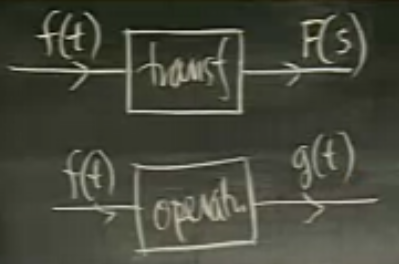
\includegraphics[height=3cm]{19_1.png}

Laplace icin kitabimizin kullandigi notasyon 

\[ \mathcal{L}(f(t)) = F(s) \]

Fakat bazen bu notasyonu kullanmak cok zor oluyor, bir suru parantez ust
uste biniyor, vs. O durumlarda su yeterli

\[ f(t) \leadsto F(s) \]

Tabii lineerlik kuralini da ustteki ile ifade etmek zor, onun icin
$\mathcal{L}$ daha iyi, 

\[ \mathcal{L}(f+g) = \mathcal{L}(f) + \mathcal{L}(g) \]

Sabitle carpim kural 

\[ \mathcal{L}(cf) = c \mathcal{L}(f)  \]

Lineerlik kurali isliyor cunku entegraller baglaminda dusunursek,
entegrallerin toplami ayni entegral altinda gruplanabilir, yani bu kural
isliyor cunku entegralin kendisi de lineer bir operator. 

Eh artik ise koyulalim. Mesela bildik bazi fonksiyonlarin Laplace
transformunu bulalim. 

Ornek

\[ 1 \leadsto ? \]

\[ \int_0^{\infty} e^{-st} \ dt \]

Dikkat, bu entegral uygun olmayan bir (improper) entegral. Bu tur
entegrallerin tanimina bakali 

\[ \lim_{R \to \infty}  \int_{0}^{R} e^{-st} dt  \]

Once su entegrali hesaplayalim, 

\[  \int_{0}^{R} e^{-st} dt \]

$t$'ye gore entegral aliyoruz, o zaman $s$ bir sabit gibidir. 

\[  = \frac{ e^{-st}}{-s}  \bigg|_{0}^{R} \]

\[ = \frac{e^{-sR} - 1}{-s} \]

O zaman 

\[ \lim_{R \to \infty}  \int_{0}^{R} e^{-st} dt  = 
\lim_{R \to \infty} \frac{e^{-sR} - 1}{-s}  = 
\frac{1}{s}
\]

Yani 

\[ 1 \leadsto \frac{1}{s} \]

Bu dogru mu? Hayir degil. Bir hata yaptik, daha dogrusu bir seyi
atladik. Limit ifadesindeki $e^{-sR}$ sifira gider, sadece ve sadece $s >
0$ ise. 
Sonucun tam hali 

\[ 1 \leadsto \frac{1}{s}, \ \ s > 0 \]

Ama diger yandan ``ya $s < 0$ ise o zaman Laplace Transformu nedir?''
sorusunun da anlami yoktur. 1'in Laplace transformu alttaki fonksiyondur,
bu fonksiyonun eksi bolgesinde karsiligi yoktur. 

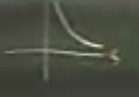
\includegraphics[height=2cm]{19_2.png}

Ornek 

\[ e^{at} \leadsto ? \]

Bu arada insanlar Laplace transform teknigini simdiye kadar pek cok
gordugumu turden fonksiyonlar uzerinde kullanirlar hep, ustel fonksiyonlar,
polinomlar, sinus, cosinus ifadeleri, kompleks sayilar, vs. Diger turden
seylerde .. onu kullanmazlar. Bu hayal kirikligi yaratmasin, ODE cozerken
Laplace teknigi bazi isleri diger kullandigimiz tekniklerden cok daha iyi
yapar. Neyse Laplace'in avantajlarina ileride daha belirgin vurgu
yapacagiz. Ornegimize donelim. 

Aslinda daha genel bir duruma bakalim, su ifadenin

\[ e^{at}f(t) \]

Laplace transformunu yapacagiz, ve bunu $f(t)$'nin transformu bilindigi
durum icin yapacagiz, ustteki blok ifade icin genel bir formul uretecegiz,
ve onu basarinca, $e^{at}$ ifadesini $e^{at} \cdot 1$ olarak gorulebilir, eh
1'in transformunu zaten biliyoruz, o zaman genel formul uzerinden $e^{at}$'in
transformunu hemen buluruz. Genel formulun transformu

\[ \int_0^{\infty} e^{at} f(t)e^{-st} \ dt \]

Iki ustel ifadeyi birlestirelim, ve oyle yapalim ki $f(t)$'in transformu
bir sekilde formulde olsun. Ulasmak istedigim nokta 

\[ \int_0^{\infty} f(t)e^{-( ... )t } \ dt \]

seklinde, eger eksi bu sekilde disarida kalacaksa, geri kalanlar neye
benzer? 

\[ \int_0^{\infty} f(t)e^{-(s-a)t } \ dt \]

Bu nedir? Bu da bir Laplace transformudur! Eger $-a$ orada olmasaydi, geri
kalanlar $f(t)$'nin transformu olacakti. O zaman 

\[ = F(s-a) \]

Sartlari koyalim, ustteki durumda $s-a > 0$ olmali, o zaman $s > a$
olmali. 

$F$ icinde $-a$ sonucu bir tur ``kaydirma'' gibi duruyor, zaten bu genel
formulun ismi ``ustel kaydirma kurali (exponential shift
law)''. Muhendisler bu kurali cok kullanirlar. 

$e^{at}$'ye donelim. 1'in transformu $1/s$ ise, kaydirma kuraliyla

\[ e^{at} \leadsto \frac{1}{s-a} \]

Peki transform edilmek istenen sinus ve cosinus oldugu durumlarda ne
yapariz? Hatirlayalim, sin ve cos ifadelerini kompleks olarak ifade
edebiliriz, ve ustteki genel kural $a$ bir kompleks sayi oldugunda da
isler. 

\[ e^{(a+bi)t} \leadsto \frac{1}{s - (a+bi)}, \ \ s>a  \]

Kontrol edelim, mesela 

\[ sin \ at \leadsto ? \]

\[ cos \ at \leadsto ? \]























\end{document}
